\documentclass[10pt,a4paper,twoside]{article}
\usepackage[english]{babel}
%laad de pakketten nodig om wiskunde weer te geven :
\usepackage{amsmath,amssymb,amsfonts,textcomp}
%laad de pakketten voor figuren :
\usepackage{graphicx}
\usepackage{float,flafter}
\usepackage{hyperref}
\usepackage{inputenc}
\usepackage{minted}
\usepackage{subcaption}

\setlength\paperwidth{20.999cm}\setlength\paperheight{29.699cm}\setlength\voffset{-1in}\setlength\hoffset{-3cm}\setlength\topmargin{1.0cm}\setlength\headheight{12pt}\setlength\headsep{0cm}\setlength\footskip{1.131cm}\setlength\textheight{25cm}\setlength\oddsidemargin{2.499cm}\setlength\textwidth{16.999cm}

\newcommand{\sweepsize}{0.24}

\pagenumbering{gobble}

\begin{document}
\begin{center}
\hrule

\vspace{.2cm}
{\bf {\Large Computer Vision - Lab Assigment Report} \\ {\Large Image segmentation}}
\vspace{.1cm}
\end{center}
{\bf Tuan Mate Nguyen}  (tunguyen@student.ethz.ch)
\hrule
\section*{Mean-shift}
First I calculated the L2 distances of the current color to all the other
pixels' color (as magnitude of the difference vector).
The implementation of the Gaussian weight function is the same for both versions
(already vectorized).
To update the current point first the color vectors of all points are multiplied
with their weights and divided by the sum of the weights (normalization). Then the
sum of these normalized color vectors yield the new color vector.

The vectorized implementation had equivalent steps exept that in the beginning I
created a copy array of all the points ($X$) for each point to allow for parallel
processing. 

\subsection*{Bandwidth}
As expected, increasing bandwidth results in fewer distinguished segmented
object. The reason is that the weights of more distant (in color-space
coordinates) colors - contained in the
image pixels -  are higher relative to closer colors' weights than in the small bandwidth case.
 As a result the mean color value assigned
to the current pixel will be closer to the global mean (mean color of the full image).
Consequently these mean values will also be closer to each other with each step until
being merged into a set of colors with only few different colors (e.g. 3 colors for $bandwidth=5$ case).

On the other hand, in case of a smaller bandwidth value, basically only the
close neighborhood would be taken into account. If the color clusters (segments) are
well-separated and far apart, then the found mean will better approximate the cluster
mean.

If, however, the bandwidth is too small, the new color will basically remain
unchanged (other colors have low weights so they have no effect) with every pixel representing a segment, resulting in an image
very similar to the original. Actually the script crashes if there are too many
colors (probably not enough labels).

\begin{figure}[h]
    \centering

    \begin{subfigure}{\sweepsize\textwidth}
    
\includegraphics[width=0.9\linewidth]{result_1.8.png} 
    \caption{$bandwidth=1.8$}
    \end{subfigure}
    \begin{subfigure}{\sweepsize\textwidth}
    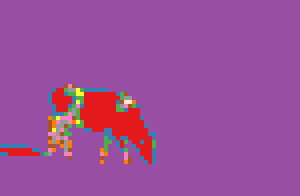
\includegraphics[width=0.9\linewidth]{result_2.5.png} 
    \caption{$bandwidth=2.5$}
    \end{subfigure}
    \begin{subfigure}{\sweepsize\textwidth}
    
\includegraphics[width=0.9\linewidth]{result_3.8.png} 
    \caption{$bandwidth=3.8$}
    \end{subfigure}
    \begin{subfigure}{\sweepsize\textwidth}
    
\includegraphics[width=0.9\linewidth]{result_5.png} 
    \caption{$bandwidth=5$}
    \end{subfigure}
    \caption{Segmented images for different bandwidth values}

\end{figure}

\subsection*{Performance}

The script was run on a desktop machine with a GeForce GTX 1080 Ti graphics
card. (note: on my laptop I got warnings about insufficient amount of RAM). The
runtime was chosen to be the fastest out of 5 measurements. As expected the CPU
version using Python loops was the slowest and the batched (vectorized) version
on the CPU was second slowest. On the GPU the non-vectorized and vecorized
implementations achieved around 2x and 16x speed-up, respectively, compared to
the best CPU result.

\begin{table}[h!]
\begin{center}
    \begin{tabular}{|c | c|} 
     \hline
     CPU & 32.41s \\
     \hline
     Batched CPU & 18.62s\\ 
     \hline
     GPU & 7.41s\\
     \hline
     Batched GPU & 1.17s\\
     \hline
    \end{tabular}
    \caption{Timing results}
\end{center}
\end{table}    

% Python code
%\begin{minted}[mathescape,
%    linenos,
%    numbersep=5pt,
%    gobble=2,
%    frame=lines,
%    framesep=2mm,
%    firstnumber=26]{csharp}
%\end{minted}

% Image
%\begin{figure}[H]
%    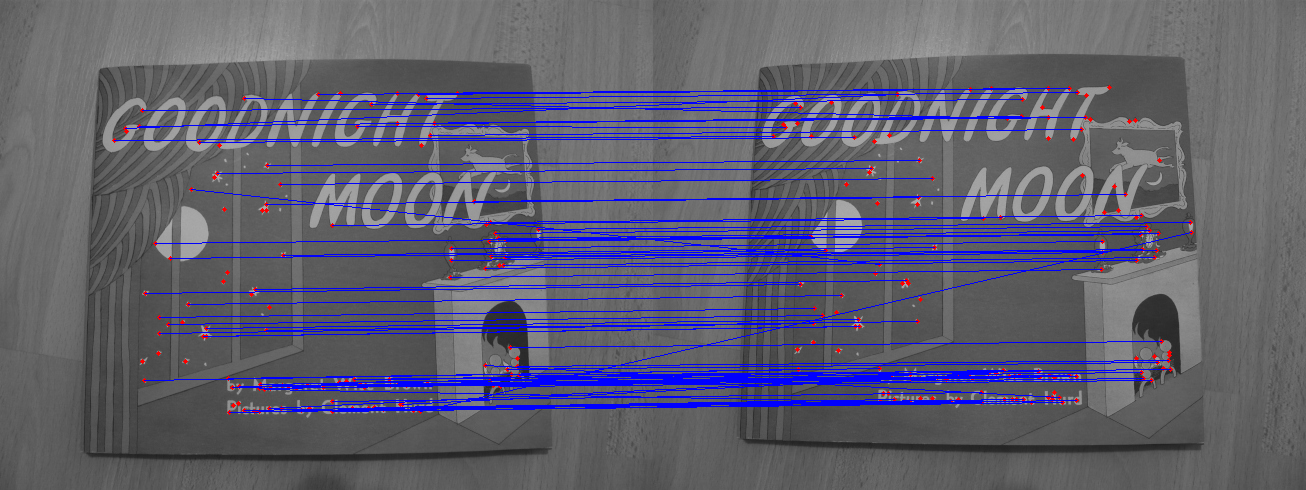
\includegraphics[width=\textwidth]{match_mutual.png}
%    \centering
%    \caption{Matching keypoints for mutual nearest neighbor matching}
%    \label{match_mutual}
%\end{figure}

\end{document}
